\subsection{Energy Shortcut Learning}
\label{sec:energy-bias}

When a deep learning classifier is trained on the datasets described in Section~\ref{sec:datasets}, it effectively has two choices: it can spend its modeling capacity learning and encoding the complex event topology, or it can resort to a simpler and more obvious feature that already distinguishes signal from background. In NLDBD datasets, energy is exactly such a feature. As shown in Figure~\ref{fig:mjd-motivation} (a), the two MJD waveforms correspond to two events with different energies: the taller waveform represents a higher-energy event, while the shorter waveform represents a lower-energy event. This energy difference is one of the most visually prominent features in the MJD dataset, and likewise among the most readily identifiable features across the other datasets.

The problem arises because signal-like and background-like events in the training set often follow different energy distributions. Figure~\ref{fig:mjd-motivation} (b) shows the normalized energy distributions of the signal-like and background-like training samples. Without learning the event topology at all, a classifier can exploit this difference with a simple ``energy cut'': classifying events above a certain energy as signal-like and events below it as background-like. As shown in Figure~\ref{fig:mjd-motivation} (c), this simple ``energy cut'' approach can already achieve an ROC AUC of 0.9706.In this case, strong classification performance does not necessarily indicate that the model has learned the underlying physics encoded in the event topology; instead, it may simply rely on energy---a simple feature that is often readily apparent by eye---and make its predictions primarily from this shortcut. We refer to this failure mode as \textbf{energy shortcut learning}.

% Strong classification performance can reflect both event morphology and
% energy-related differences between classes. Energy is valid physical
% information, but comparisons intended to assess structure beyond energy
% should also control the class energy spectra. Otherwise, accessible energy
% cues can provide a shortcut relative to that objective
% \citep{geirhos2020shortcut}.

% MJD provides a concrete example. Its benchmark distinguishes clean events,
% which pass all four reference pulse-shape cuts, from non-clean events.
% Pulse height is approximately related to calibrated energy in the released
% waveforms~\citep{majorana_ml_dataset}. Our classification preprocessing
% subtracts the mean of the first 200 samples and divides each waveform by
% its maximum absolute amplitude. Although this removes the leading amplitude
% scale, it need not remove energy information from the remaining waveform.

% Figure~\ref{fig:mjd-motivation} compares low- and high-energy clean events
% from the same detector and run. Across all 410 clean test events in this
% group, the median normalized baseline RMS is 7.56 times larger in the
% lowest than in the highest energy quartile, with 103 events per cohort.
% The association is also visible across the full group
% (Spearman $\rho=-0.826$). Thus relative noise can carry an energy cue after
% amplitude normalization, even with the true class, detector, and run held
% fixed. The waveform precedes the model-specific representation adapter;
% this diagnostic does not establish which cues a trained classifier uses.

% The clean and non-clean test populations have different energy spectra.
% Together, these observations motivate evaluating discrimination after
% balancing class energy distributions and separately testing the energy
% dependence of predictions. Appendix~\ref{app:mjd-motivation} gives the
% selection rule and normalization details. SuperNEMO supplies a complementary
% example of energy-associated tracker geometry
% (Appendix~\ref{app:raw-observations}).

\begin{figure}[!htb]
\centering
    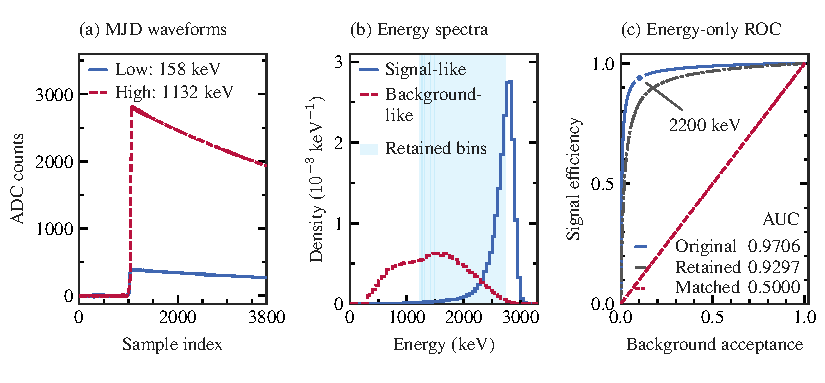
\includegraphics[width=\linewidth]{wing_contribution/figures/mjd_motivation_main_v2_generated.pdf}
\caption{Energy shortcuts in detector data.
(a) Baseline-subtracted MJD waveforms from two clean test events with energies of 158 and 1132\,keV.
(b) Unit-area energy spectra for SuperNEMO $0\nu\beta\beta$ (signal-like) and $^{214}$Bi (background-like) test events. Shading marks retained 5\,keV matching bins; spectra use 50\,keV display bins.
(c) ROC curves using energy alone as the score for the original population, retained events with unit weights, and the same retained events after matching. The point marks a 2200\,keV threshold.}
\label{fig:mjd-motivation}
\end{figure}

